\subsection{Filters and Estimators comparison}
\label{subsec:comparison_filters}

In this section, we compare the filters and estimators designed in Section \ref{sec:filters_estimators_design}, using an LQR tracking controller to assess their ability to track the system's state during continuous oscillatory motion.

The primary objective is to evaluate the effectiveness of each filtering method in ensuring accurate tracking of the sphere's trajectory relative to the sinusoidal reference, as well as the quality of the resulting control signal.

To achieve this, a continuous sinusoidal reference signal with a period of 6 seconds is used.
This setup allows us to analyze the filters' performance in handling gradual oscillations.
As in the sinusoidal input used for the controllers comparison, the oscillations range between $12 [mm]$ and $8 [mm]$.

The following figures illustrate the performance of the filters and estimators in tracking the system's state under these oscillatory conditions.

\begin{figure}[H]
    \centering
    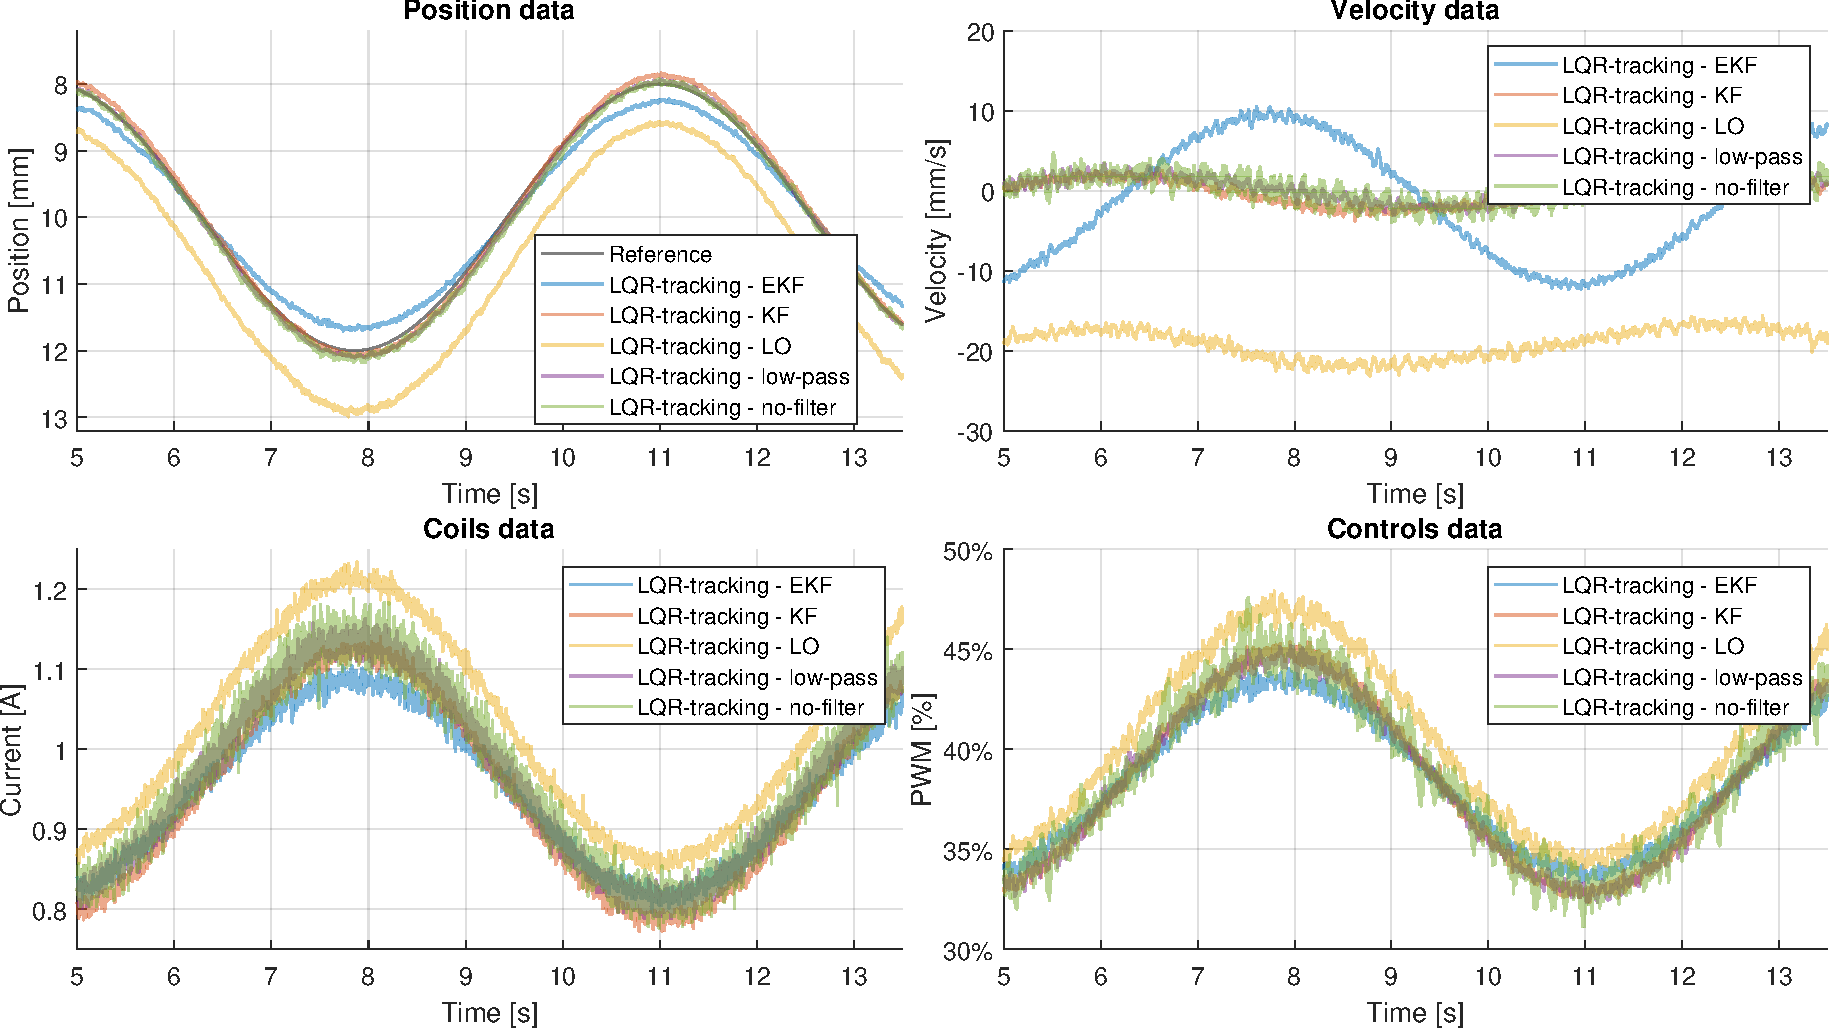
\includegraphics[width=1\linewidth]{./img/MATLAB/results/sinusoidal_slow_linear_star_star.pdf}
    \caption{Comparison of filter using an LQR tracking with sinusoidal slow reference}
\end{figure}

\begin{figure}[H]
    \centering
    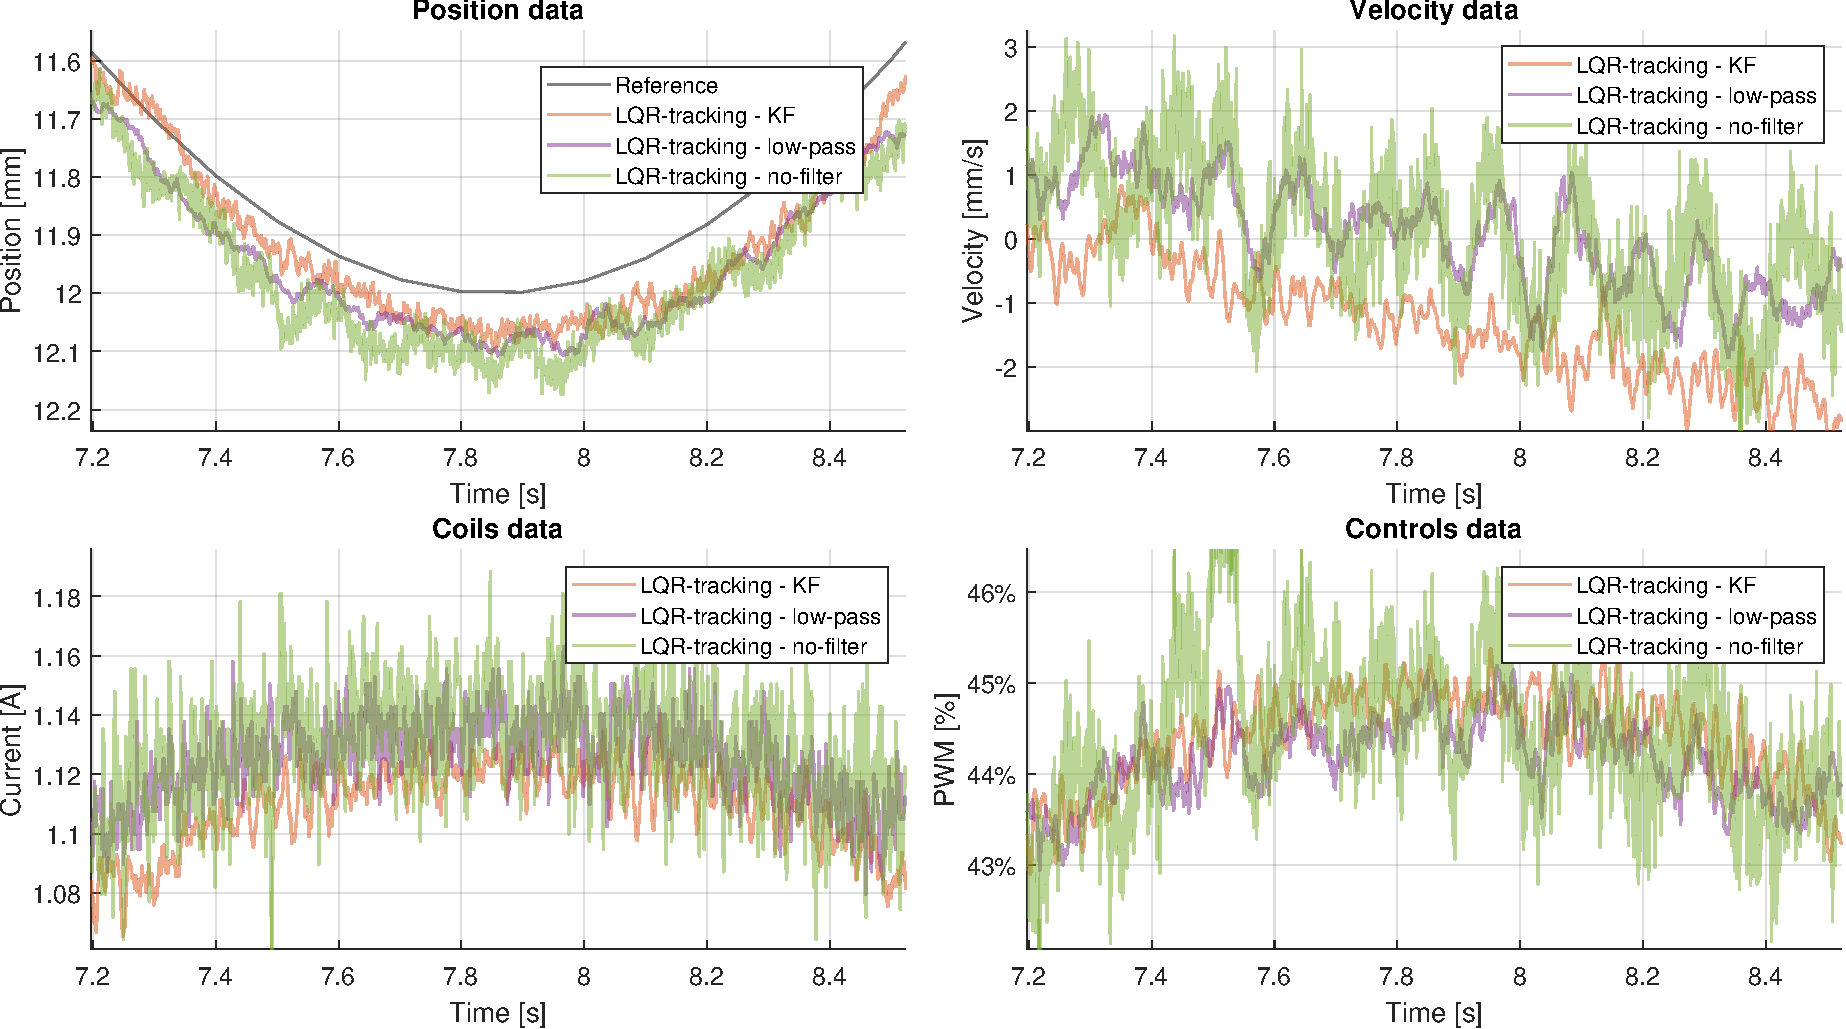
\includegraphics[width=1\linewidth]{./img/MATLAB/results/sinusoidal_slow_linear_zoomed_star_no_filter_low_pass_KF.pdf}
    \caption{Comparison of no filter, low pass, KF using an LQR tracking with sinusoidal slow reference}
\end{figure}


\paragraph{Raw measurements}

Clearly due to the absence of filtering, the system noise is not reduced.
Noise filtering, especially for velocity, is critical to achieving accurate response.
Using the controller without filters results in the least precise trajectory tracking.

The control performance is visibly affected by oscillations, making this approach not optimal for the system under consideration.

\paragraph{Low pass filter}

Introducing a low pass filter improves the response accuracy compared to the unfiltered case.

However, its ability to eliminate noise is limited by the filter's non-adaptive nature, which hinders dynamic performance.
The accuracy is higher respect to the case without filters, but lower respect to the other filters except for the Luenberger observer.

\paragraph{Luenberger observer (LO)}

This case represents the least effective way to estimate the state.

The Luenberger observer can be worse than the unfiltered case because it uses a non-optimal fixed-gain feedback, amplifying the noise and introducing errors in the state estimation.
Furthermore, by not handling stochastic noise statistically, it compromises the control, which in this case is less precise than using the noisy measurements directly.

\paragraph{Standard Kalman filter (KF)}

The Kalman filter emerged as the most effective method among those tested.

Its ability to optimize state estimation in the presence of measurement and process noise significantly enhances control quality.
As a consequence, the control signal is more accurate and less noisy, leading to improved system performance.
The trajectory tracking exhibited the highest accuracy with minimal oscillations.

\paragraph{Extended Kalman filter (EKF)}

Although the EKF is designed to handle system non-linearities, the results showed inferior performance compared to the standard Kalman filter.
Specifically, the EKF failed to adequately follow the reference trajectories.

This could be attributed to suboptimal linearizations or poorly tuned covariance matrices.
These findings suggest that applying the EKF requires further investigation and optimization to achieve competitive performance.


\subsubsection{Conclusions}
\label{subsubsec:conclusions_filters_comparison}

The comparative analysis highlighted a clear hierarchy in the performance of the various approaches.

The standard Kalman filter stands out as the optimal solution for the analyzed system, ensuring precise and stable control.
In contrast, the Luenberger observer is the least effective way to filter.
Despite its theoretical potential, the EKF delivered unsatisfactory results compared to its simpler counterpart, indicating that further tuning is required.

% These results underscore the importance of selecting appropriate filters.
